\section{Engineering of a novel tri-functional enzyme with MnSOD, catalase 	and cell-permeable activities}

\subsection{Нормальное название}

Разработка нового полифункционального фермента, способного проникать в клетки млекопитающих, обладающего супероксиддисмутазной и каталазной активностями.

\subsection{Абстракт}

Кооперативное действие супероксиддисмутазы(SOD) и каталазы (CAT), проявляющееся в защите от окислительного стресса, является более эффективным, чем действие каждого из этих ферментов в отдельности. Химическая конъюгация этих двух ферментов позволяет получить молекулу с более высокой антиоксидантной активностью и, следственно, терапевтической эффективностью. Однако у химических методов сшивания белков есть следующие недостатки: потеря энзиматической активности, низкая гомогенность полученных продуктов, трудоемкость и необходимость очистки продукта от использованных реактивов. Тем не менее, не было доказано, что химически конъюгированные ферменты способны функционировать в заданных клетках-мишенях. В этом исследовании с помощью генной инженерии авторы впервые сконструировали и синтезировали бифункциональный фермент с супероксиддисмутазной и каталазной активностями. Чтобы позволить ферменту функционировать в клетке, был использован пептид Tat вируса иммунодефицита человека (ВИЧ), способный проникать через клеточную мембрану. Совместная экспрессия генов каталазы с супероксиддисмутазой (марганецсодержащей) и ТАТ привела к спонтанной самосборке аминокислотных последовательностей в крупный белковый комплекс. В его состав предполагаемо входят следующие структурные элементы: один тетрамер каталазы,четыре тетрамера марганцевой супероксиддисмутазы и двенадцать мономеров белка ТАТ. Белок был помещен внутрь клетки и продемонстрировал поразительную защитную реакцию на вызываемую паракватом клеточную гибель (по сравнению с отдельными ферментами или комплексом без ТАТ). Это исследование не только предлагает альтернативную стратегию синтеза мультифункционального белкового комплекса, но также иллюстрирует возможность для дальнейшего изучения агентов для терапии окислительного стресса и связанных с ним состояний.

\subsection{Картинки}

\begin{figure}[H]
	\centering
	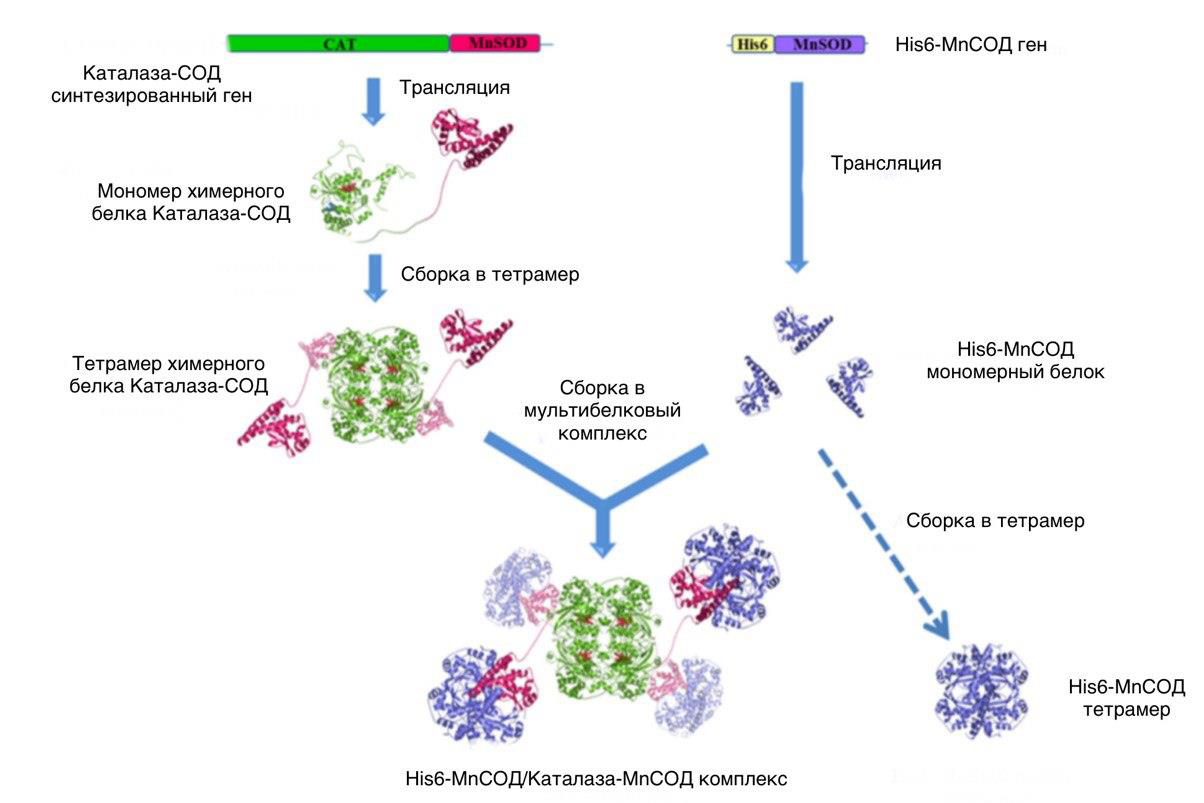
\includegraphics[width=\linewidth]{181_12_1}
	\caption{Схематическое изображение стратегии конструирования бифункционального белка с супероксиддисмутазной и каталазной активностями. Совместная экспрессия химерного гена CAT-MnSOD с геном 6His-MnSOD позволяет получить мономер белка CAT-MnSOD и 6His-MnSOD. Затем два мономера собираются в большой мультимерный комплекс M/CM белков или в тетрамер 6His-MnSOD. Для получения трифункционального белка с функциями MnSOD и каталазы, а также способного проникать в клетку, ген 6His-MnSOD был заменен на химерный ген 6His-MnSOD-TAT.}
	\label{fig:181_12_1}
\end{figure}


\begin{figure}[H]
	\centering
	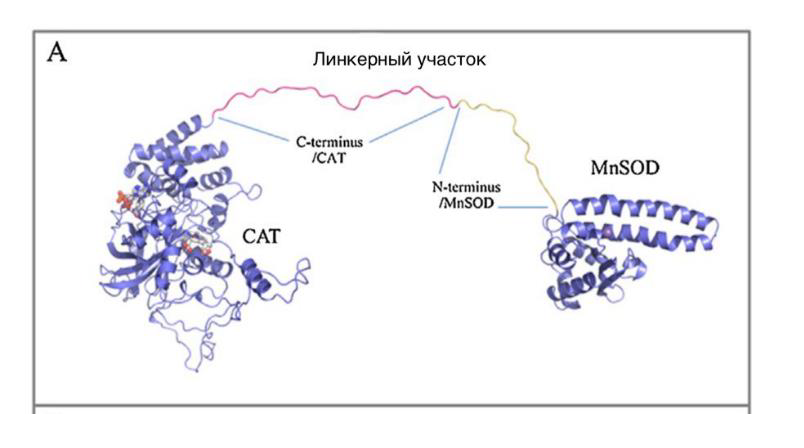
\includegraphics[width=\linewidth]{181_12_2A}
	\caption{Структурная модель химерного белка CAT-MnSOD (А). Модель одиночной цепи CAT-MnSOD. Линкер включает последние двадцать шесть C-концевых остатков 502-527 CAT и первые пятнадцать N-концевых остатков MnSOD}
	\label{fig:181_12_2A}	
\end{figure}


\begin{figure}[H]
	\centering
	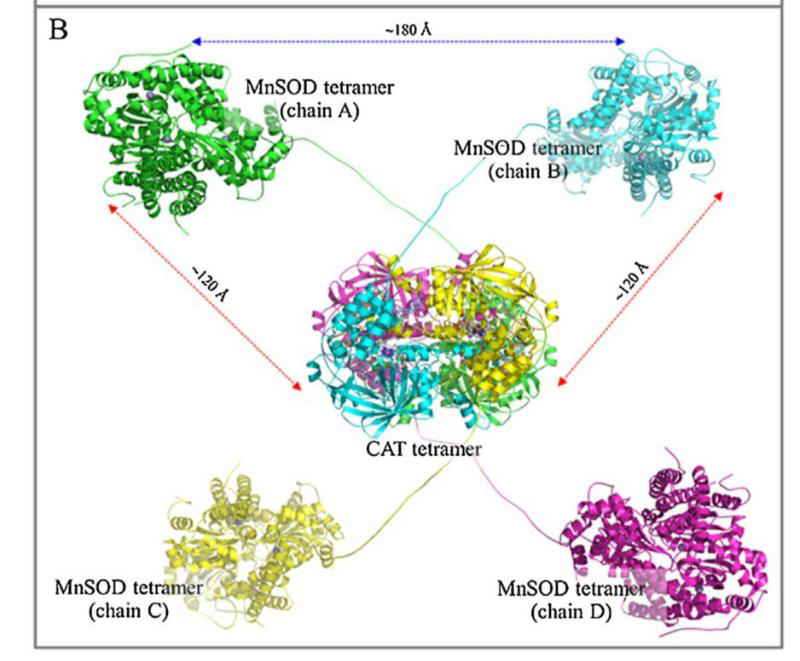
\includegraphics[width=\linewidth]{181_12_2B}
	\caption{(В). Модель тетрамерного CAT-MnSOD, построенная в соответствии с кристаллической структурой тетрамерной CAT человека (код pdb 1DGF). Определены расстояния до центра масс между MnSOD и CAT, а также между каждым соседним MnSOD. Гетероатомы, включая ионы гема, НАД и иона Mn3 +, показаны в шаровой модели.}
	\label{fig:181_12_2B}		
\end{figure}


\begin{figure}[H]
	\centering
	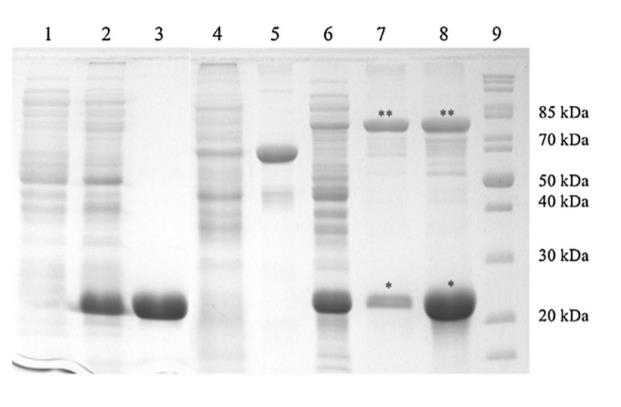
\includegraphics[width=\linewidth]{181_12_3}
	\caption{Экспрессия и очистка нативных и химерных белков. Очищенные белки определяли с помощью электрофореза в ПААГ. Дорожка 1: неочищенный экстракт белков E. coli, несущий контрольную плазмиду pETDuet-1, дорожка 2: неочищенный экстракт белков E. coli, несущий pET46-MnSOD, дорожка 3: очищенный 6His-MnSOD, дорожка 4: неочищенный экстракт белков E. coli, несущий pET46-CAT, дорожка 5: очищенный 6His-CAT, дорожка 6: неочищенный экстракт белков E. coli, несущий pETDuet-MnSOD / CATMnSOD, дорожка 7: очищенный с помощью гель-фильтрационной хроматографии комплекс M/CM, дорожка: IMAC-очищенный белок, полученный в результате совместной экспрессии 6His-MnSOD и CM, дорожка 9: маркер молекулярной массы белка (* обозначает 6His-MnSOD и ** обозначает химерный белок CM).}
	\label{fig:181_12_3}		
\end{figure}

\begin{figure}[H]
	\centering
	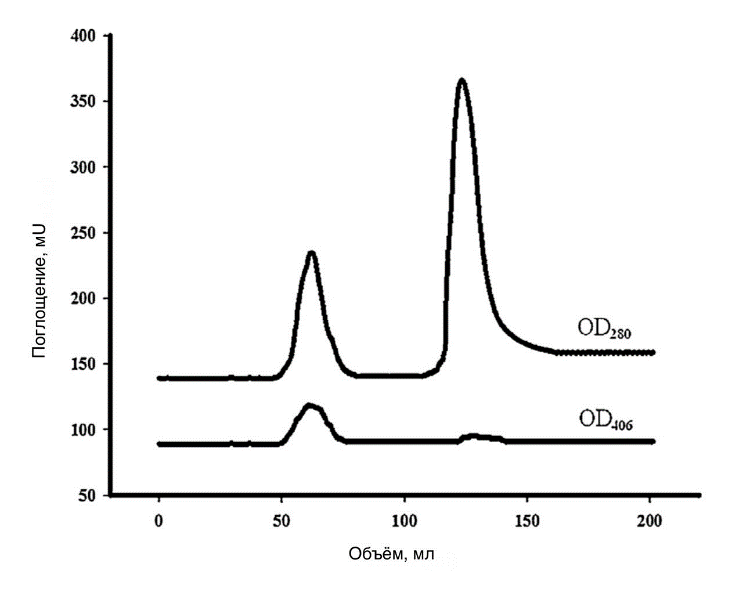
\includegraphics[width=\linewidth]{181_12_4}
	\caption{Хроматограмма гель-фильтрационной хроматографии, выполненной на колонке для гель-фильтрации Sephacryl S300HR. Разделенные пики белков 6His-MnSOD и комплекса M/CM определяли по поглощению при 280 нм, а присутствие гема простетической группы отслеживали с помощью поглощения при 406 нм.}
	\label{fig:181_12_4}		
\end{figure}

\begin{figure}[H]
	\centering
	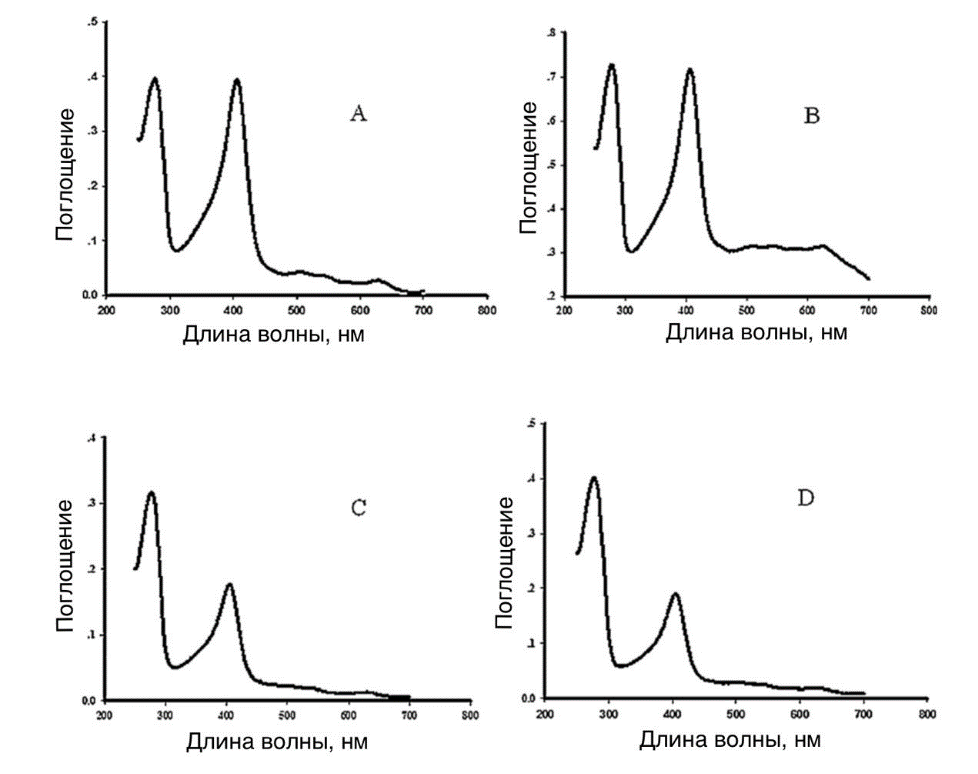
\includegraphics[width=\linewidth]{181_12_5}
	\caption{Спектры поглощения очищенных белков (250–700 нм). Пик поглощения гема представлен при 406 нм. 6His-CAT (A); 6His-CAT-TAT (B); M/CM (C) и M-TAT/CM (D).}
	\label{fig:181_12_5}		
\end{figure}


\begin{figure}[H]
	\centering
	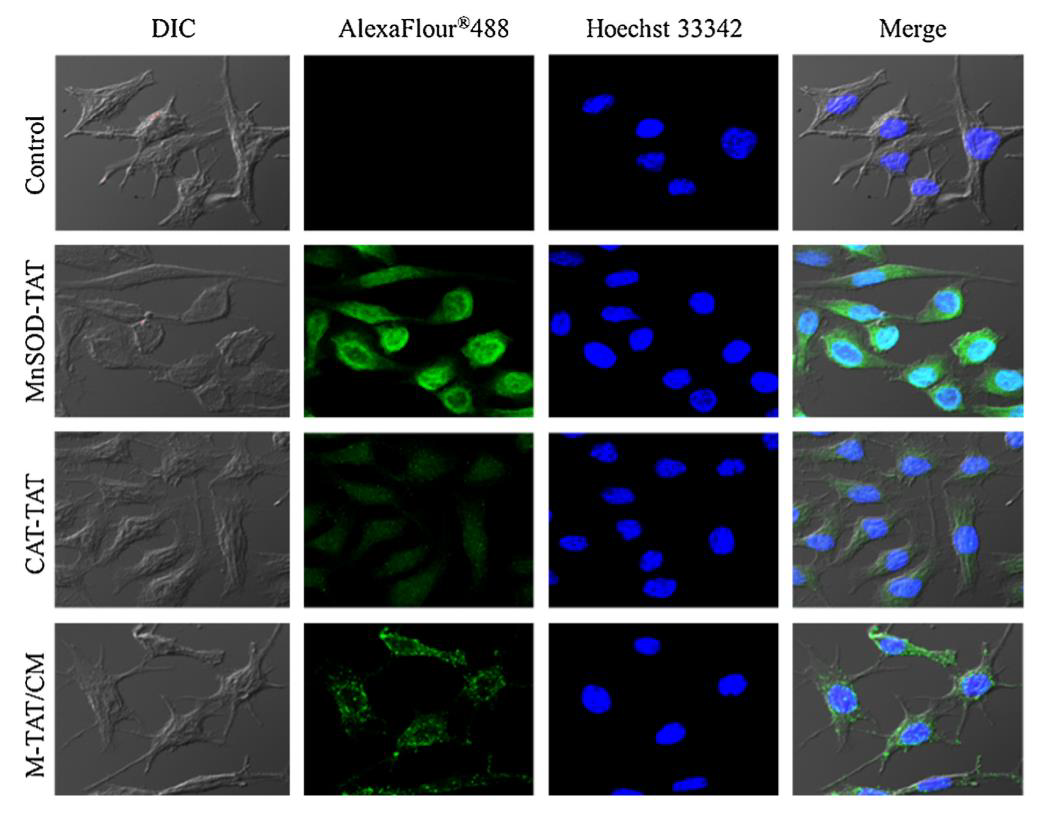
\includegraphics[width=\linewidth]{181_12_6}
	\caption{Проникновение в клетки L929 6His-CAT-TAT, 6His-MnSOD-TAT и M-TAT/CM, меченных Alexa Flour 488®. Исследование и визуализация с помощью конфокальной микроскопии. Изображения были получены после обработки клеток L929 0,1 М раствором целевых белков в течение 1 часа. Ядра клеток окрашены Hoechst 33342.}
	\label{fig:181_12_6}		
\end{figure}

\begin{figure}[H]
	\centering
	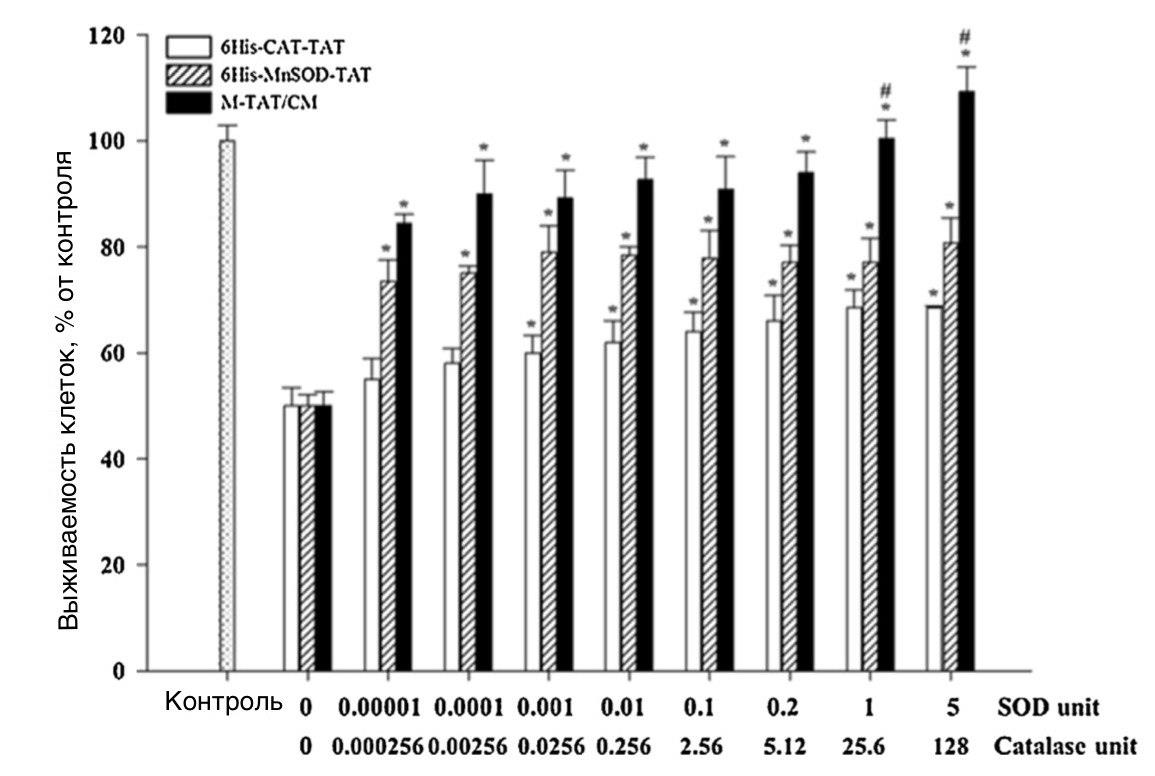
\includegraphics[width=\linewidth]{181_12_7}
	\caption{Защитный эффект гибридных белков на оксидативный стресс, вызванный паракватом, в клетках L929. Клетки предварительно обрабатывали различными единицами белков в течение 1 часа. После удаления избытка белка клетки промывали и инкубировали с 30 мМ паракватом в течение 5 часов. Жизнеспособность клеток исследовали с помощью анализа MTS. Данные выражены как среднее значение ± стандартное отклонение в трех независимых экспериментах. Статистический анализ оценивали с помощью парного t-критерия, p-value < 0.05.}
	\label{fig:181_12_7}		
\end{figure}